%        File: VTthesis_template.tex
%     Created: Thu Mar 24 11:00 AM 2016 EDT
%     Last Change: Mon, April 30, 2018
%      Author: Alan M. Lattimer, VT
%	   With modifications by Carrie Cross, Robert Browder, and LianTze Lim.
%
% This template is designed to operate with XeLaTeX.
%
% All elements in the Title, Abstract, and Keywords MUST be formatted as text and NOT as math.
%
%Further instructions for using this template are embedded in the document. Additionally, there are comments at the end of the file that give suggestions on writing your thesis.
%
%In addition to the standard formatting options, the following options are defined for the VTthesis class: proposal, prelim, doublespace, draft.

\documentclass[nopageskip,prelim]{VTthesis} % nopageskip = Removes arbitrary blank pages.

\usepackage{microtype} % Not everything is supported when using XeLaTeX, but should help a bit in making text look nicer.
\usepackage{textcomp}  % Fixes issue with microtype+siunitx's \micro

\usepackage[en-US]{datetime2}      % For \DTMdate, etc.
\usepackage[binary-units]{siunitx}
\usepackage{mathtools}             % for \coloneqq
\usepackage{bussproofs}            % for prooftree environment

\usepackage{booktabs}              % For nicer-looking tables
\usepackage{makecell}              % For table heading cells and cells with line breaks
\usepackage{threeparttable}        % For tables with notes

\usepackage[index,single]{acro}                  % For acronyms; hyperref option changes acro colors but doesn't actually link to the list so not using it right now
\usepackage{makeidx}               % For indices!
\usepackage{cleveref}              % Better auto-reference-typing than \autoref{}

\usetikzlibrary{graphs}            % dot-style graph shorthands (not quite as compactible as dot language, though)
\usetikzlibrary{quotes}            % needed for quoted edge labels (only in graphs?)

\renewcommand\lstlistlistingname{List of Listings}

\DeclareAcronym{abi}{
  short            = ABI,
  short-indefinite = an,
  long             = application binary interface,
  long-indefinite  = an
}
\DeclareAcronym{cfg}{short=CFG, long=control flow graph}
\DeclareAcronym{ipc}{
  short            = IPC,
  short-indefinite = an,
  long             = inter-process communication,
  long-indefinite  = an
}
\DeclareAcronym{isa}{
  short            = ISA,
  short-indefinite = an,
  long             = instruction set architecture,
  long-indefinite  = an
}
\DeclareAcronym{os}{
  short            = OS,
  short-indefinite = an,
  long             = operating system,
  long-indefinite  = an,
  short-plural     = es
}
\DeclareAcronym{sloc}{short=SLOC, long=source lines of code}
\DeclareAcronym{sse}{
  short            = SSE,
  short-indefinite = an,
  long             = Streaming SIMD Extensions,
  long-indefinite  = an,
}
\DeclareAcronym{tcb}{short=TCB, long=trusted computing base}
\DeclareAcronym{vm}{short=VM, long=virtual machine}

\lstdefinelanguage
  [x64]{Assembler}     % add an "x64" dialect of Assembler
  [x86masm]{Assembler} % based on the "x86masm" dialect
  % with these extra keywords:
  {morekeywords={CDQE,CQO,CMPSQ,CMPXCHG16B,JRCXZ,LODSQ,MOVSXD,% will add more insts as needed
      POPFQ,PUSHFQ,SCASQ,STOSQ,IRETQ,RDTSCP,SWAPGS,%
      MOVAPD,MOVDQA,
      dil,%
      rax,rdx,rcx,rbx,rsi,rdi,rsp,rbp,rip,%
      r8,r8d,r8w,r8b,r9,r9d,r9w,r9b,%
      r10,r10d,r10w,r10b,r11,r11d,r11w,r11b,%
      r12,r12d,r12w,r12b,r13,r13d,r13w,r13b,%
      r14,r14d,r14w,r14b,r15,r15d,r15w,r15b}} % etc.
\lstdefinestyle{x64}{
  language=[x64]{Assembler},
  keywordstyle=\bfseries\color{blue}, % bold blue keywords
  commentstyle=\color{gray},
  identifierstyle=\color{purple},
  stringstyle=\color{brown},
}

\newcommand{\inlineasm}[1]{\lstinline[style=x64]|#1|}

%% Math commands
\newcommand{\var}[1]{\mathit{#1}}
\DeclareMathOperator{\step}{step}
\DeclareMathOperator{\run}{run\_until}
\DeclareMathOperator{\loc}{loc}

\newcommand{\region}[2]{\ensuremath{[#1,#2]}}
\newcommand{\readmem}[2]{\ensuremath{\ast\region{#1}{#2}}}
\newcommand{\readmemS}[3]{\ensuremath{#1:\readmem{#2}{#3}}}
\newcommand{\htriple}[3]{\{#1\}~#2~\{#3\}}

\newcommand{\deqptr}{\var{deq}_\mathrm{ptr}}
\newcommand{\bufferptr}{\var{buf}_\mathrm{ptr}}
\newcommand{\outptr}{\var{out}_\mathrm{ptr}}
\newcommand{\valueptr}{\var{value}_\mathrm{ptr}}

\newcommand{\mathrip}{\text{\inlineasm{rip}}}
\newcommand{\mathrbp}{\text{\inlineasm{rbp}}}
\newcommand{\mathrbx}{\text{\inlineasm{rbx}}}
\newcommand{\mathrdi}{\text{\inlineasm{rdi}}}
\newcommand{\mathrsi}{\text{\inlineasm{rsi}}}
\newcommand{\mathrsp}{\text{\inlineasm{rsp}}}
\newcommand{\mathdil}{\text{\inlineasm{dil}}}
\newcommand{\mathdl}{\text{\inlineasm{dl}}}

\newcommand{\rspo}{\var{rsp}_0}
\newcommand{\rbpo}{\var{rbp}_0}

\newcommand{\retaddr}{\mathtt{ret\_addr}}

% Misc. commands
\newcommand{\todo}[1]{{\bfseries\color{purple}#1}} % Allowing paragraphs in todos
\newcommand*{\fturl}[1]{\footnote{\url{#1}}}

% Title of your thesis
\title{Title of your thesis goes here}

% You should include 3-5 keywords, separated by commas
\keywords{Some Keywords, Subject matter, etc.}

\author{Joshua A. Bockenek}
\program{Electrical and Computer Engineering}

% Change this to your degree, e.g. Master of Science, Master of Art, etc.
\degree{Doctor of Philosophy}

% This should be your defense date: (update when settled)
\submitdate{\DTMdate{2019-09-01}}

% Committee members. Only have five readers and one chair available.
% Only use the ones you need and don't include the ones you don't need.
% Per the VT ETD standards,
% you should not include titles or educational qualifications such as PhD or Dr.
% You should, however, include middle initials if possible.
\principaladvisor{Binoy Ravindran}
\firstreader{x}
\secondreader{x}
\thirdreader{x}
\fourthreader{x}
\fifthreader{x}

% The dedication and acknowledgement pages are optional. Comment them out to remove them.
\dedication{This is where you put your dedications.}
\acknowledge{This is where you put your acknowledgments.}

% The abstract is required and should be <=250 words for thesis, <=350 words for dissertation.
\abstract{Give a brief description of your thesis here. Max of 250 words for a master's thesis and 350 words for a PhD dissertation, according to the VT ETD standards.}

% The general audience abstract is required. There are currently no word limits.
\abstractgenaud{You are also required as of Spring 2016 to include a general audience abstract. This should be geared towards individuals outside of your field that may be reading seeking information about your work. You should avoid language that is particular to your field and clearly define any terms that may have special meaning in your discipline.}

\makeindex
\begin{document}
  % The following lines set up the front matter of your thesis or dissertation and is required to ensure proper formatting per the VT ETD standards.
  \frontmatter
  \maketitle
  \tableofcontents

	\listoffigures
  \listoftables
  % Bit of work needed to get listings and acronyms in the TOC properly
  \clearpage\phantomsection % Getting hyperref to link to the right page
  \addcontentsline{toc}{chapter}{\lstlistlistingname}
  \lstlistoflistings
  \clearpage\phantomsection % Getting hyperref to link to the right page
  \addcontentsline{toc}{chapter}{Acronyms}
  \printacronyms[heading=chapter*]
  \printnomenclature

  % The following sets up the document for the main part of the thesis or dissertation. Do not comment out or remove this line.
	\mainmatter

  \chapter{Introduction}
  \section{Levels of Verification}
  \section{Challenges of Assembly-Level Verification}

  \chapter{Related Work}
  \section{Restrictions on Supported Features}
  \section{Previous Approaches to Assembly Verification}

  \chapter{Background}\label{ch:background}
This part of my dissertation provides domain-specific information necessary to understand
the work presented in it.

\section{Formal Methods}
To quote \textcite{butler:fm},
\todo{should go in intro maybe}
\begin{quote}
  ``Formal Methods''%
  \index{formal!methods}
  refers to mathematically rigorous techniques and tools
  for the specification, design and verification of software and hardware systems.
\end{quote}
This dissertation comes under the \emph{verification} component of that,%
\index{formal!verification}

\subsection{Semantics}
Very often when working with formal tools, you must formulate formal semantics
for a language.

\subsubsection{Operational}
\paragraph{Big-Step}
\paragraph{Small-Step}

\subsubsection{Denotational}

\subsubsection{Axiomatic}
Axiomatic semantics provide meaning 
The canonical example is \emph{Hoare logic}.%
\index{Hoare!logic}

\subsection{Fixed Point Representation}
The \ac{lfp} and \ac{gfp} of a function are

\todo\dots

The \ac{lfp} of an infinite loop formulated in this way
is thus the bottom element $\infloop$.%
\nomenclature{$\infloop$}{Indicates non-terminating state}

\subsection{Symbolic Execution}
At its most basic, ``symbolic execution'' refers to
executing a program with a set of symbolic inputs
rather than concrete values \autocite{king1976symbolic}.
Based on the semantics of the program, the execution may end up taking multiple paths;
it could potentially be an infinite number if there are loops involved.

\todo{more}

\todo{The below doesn't really sound right.}
In this work, the individual steps of symbolic execution
are implemented as \emph{rewrite rules} over the state%
\index{symbolic execution!rewrite rule}
that derive their representation from 
Applying those rules in sequence to each step or instruction of a program
allows aggregation of the individual state changes involved in the execution.

\subsection{Floyd Flowcharts}\label{se:floyd}

\subsection{Hoare Logic}\label{se:hoare}
A form of \emph{axiomatic semantics},
\index{semantics!axiomatic}
Hoare logic \autocite{hoare1969axiomatic,myreen2007hoare}%
\index{Hoare!logic}
describes the behavior of a program
in terms of a set of rules that are applied iteratively
in order to syntactically decompose the program into its constituent behaviors.

A \emph{Hoare triple} denotes a pre- and postcondition for a certain program.%
\index{Hoare!triple}%
\index{precondition}%
\index{postcondition}
Let~$P$ and~$Q$ be state predicates.

\todo{more}

\subsubsection{Verification Condition Generation}
%TODO

There are two ways of performing verification condition generation%
\index{verification condition generation}:
either start at the end and go backwards, deriving the \emph{weakest precondition},%
\index{precondition!weakest}
or start at the front and go forwards, deriving the \emph{strongest postcondition}.%
\index{postcondition!strongest}
The weakest-precondition approach appears most common,
being the canonical methodology.\todo{need citation}

%TODO

\subsection{Theorem Proving}
%
\index{theorem prover}

\subsubsection{Automated versus Interactive}
\index{theorem prover!interactive}

\subsubsection{Isabelle and HOL}
The theorem prover utilized in this work
was Isabelle 2018\fturl{https://isabelle.in.tum.de/} \autocite{nipkow2002isabelle}.%
\index{Isabelle/HOL}
It is a generic tool with a flexible, extensible syntactic framework.
Isabelle also utilizes a powerful proof language
known as \ac{isar}  \autocite{wenzel2007isabelle}
and a proof method language called Eisbach \autocite{matichuk2016eisbach}.
We made heavy use of Isabelle's Word library  \autocite{isabelle-word-session}
for the work presented in this dissertation.
That library provides a limited-precision integer type, \lstinline|'a word|,
where \lstinline|'a| is the number of bits in the integer.
Various operations are provided for manipulation of and arithmetic involving formal words,
including bit indexing, bit shifting, setting specific bits,
and signed and unsigned arithmetic.
Operators for inequality are also included,
as well as operations for converting between word sizes.

\paragraph{Eisbach}
\todo{explain basic steps, how +, ?, commas, etc. work and all}

%\todo{this is redundant with the info presented in symb exec}
%In order to perform symbolic execution of assembly instructions in Isabelle,
%the instructions must somehow be embedded in the theorem prover.
%This is done using the symbolic execution toolchain
%of \textcite{roessle2019},
%the \emph{machine model} of which is based on the work of \textcite{heule2016stratified}.%
%\index{symbolic execution!machine model}

%
\index{embedding!shallow}%
\index{embedding!deep}

\section{Assembly Language}
\todo\dots

The x86-64
\index{x86-64}
\ac{isa}, originally

\subsection{Basic Blocks}
Much of the memory work in this document relates to the concept of \emph{basic blocks}.%
\index{basic block}
A basic block is defined here as a sequence of assembly instructions
whose behavior can be described using only state transitions and branches.
A block always terminates and has no internal loops.
This definition differs slightly from the definition used by compilers such as LLVM,
in which basic blocks have the additional restriction that
each block must terminate with a control flow instruction and contain no other
control flow instructions.

\section{Summary}

  \chapter{Memory Usage}\label{ch:memory}
This chapter provides an introduction to the concept of \emph{memory usage}.%
\index{memory!usage}

\todo{more}

\section{Definitions}
Much of the memory work in this document relates to the concept of
\emph{basic blocks}.\index{basic block}
A basic block is defined here as a sequence of assembly instructions
whose behavior can be described using only state transitions and branches.
A block always terminates and has no loops.
This definition differs slightly from the definition used by compilers such as LLVM,
in which basic blocks also do not contain any internal branching.

\subsection{Memory Regions}\label{memory_regions}
%
\index{memory!region}



\section{Memory Region Relations}\label{mem_reg_rel}
%
\index{memory!region!relation}

\section{Memory Preservation}\label{se:memory_preservation}
An application of memory usage analysis,
memory preservation shows that the values written by a program%
\index{memory!preservation}
are restrained to specified regions in memory.
Those regions cannot be fully identified when working with source code alone,
particularly when the end result is optimized.
Memory may be laid out differently depending on the \ac{isa} and \ac{abi} targeted,
as well as on the compiler used.
This can include positioning of global variables
as well as the layout of stack frames.\index{stack!frame}
While one way of resolving that issue would be to choose a specific compiler
and provide a formal analysis of how it arranges memory, that method is not flexible.
It may instead be better to target assembly or machine code directly,
as done in this dissertation.

\subsection{Usefulness}
The following small sections elaborate on the usefulness of memory preservation
as a platform for further verification efforts.

\subsubsection{Security}
Unbounded memory usage can lead to vulnerabilities
such as buffer overflows and data leakage.
One example of such a vulnerability would be 2014's Heartbleed~\citep{heartbleed}.
Heartbleed was caused by a lack of bounds checking on a string array
requested as output as part of a ``heartbeat'' message.
This, combined with a custom memory manager
that also had no security protections against out-of-bounds memory accesses,
lead to potential leakage of sensitive data such as passwords and encryption keys.
% TODO: need another, better example that involves data modification too
Memory preservation can serve as a foundation for formal security analyses%
\index{memory!preservation}
that could be used to expose vulnerabilities involving malicious writes.

\subsubsection{Composition}\label{sse:composition}
Scalability in verification is only feasible with composition.%
\index{scalability}%
\index{formal!verification}
Proofs of functional correctness over a large suite of software
require decomposing that suite into manageable chunks.
Separation logic provides a \emph{frame rule} that supports such%
\index{separation logic}%
\index{separation logic!frame rule}
decomposition~\citep{o2001local,reynolds2002separation,krebbers2017essence}.
In words, the frame rule states that,
if a program or program fragment can be confined to a certain part of a state,
properties of that program or program fragment carry over
when used as part of a larger system involving that state.
Memory preservation allows for discharging the most involved part of the frame rule,
at least in terms of individual assembly functions.
That is, it shows that the memory usage of those functions is constrained
to specific regions in memory.
This can then serve as a basis
for any larger proof effort over multifunction assembly programs.

\subsubsection{Concurrency}
Reasoning over concurrent programs is complicated
due to the potential interactions between threads.
While there are ways of handling such interactions in a structured manner
via kernel- or library-provided \ac{ipc},
one method commonly used for the sake of efficiency is \emph{shared memory}.
Shared memory, in the context of this work,
refers to threads or processes sharing either a full memory space
or portions of one (via memory mapping)
that can be written to and read from freely by any thread or process with access to it.
Usage of shared memory can result in \emph{unintended} interactions between threads.
Memory preservation could be adapted to show the absence of such interactions
by proving that multiple threads only write
to specifically-allowed regions of shared memory.
Doing so would, of course, require a proper model of concurrency,
which is out of scope of this dissertation.

\subsection{Formal Definition}
The formal definition of memory preservation takes the form of a Hoare triple.%
\index{memory!preservation}%
\index{Hoare!triple}
Initially, there must be some predicate~$P$ that characterizes the initial state,
at a minimum by setting the instruction pointer
to the first instruction of the relevant function body.
In addition, $M$ is the set of regions in memory
that the function is allowed to write to.
Set~$M$ includes the stack frame and any utilized data sections from the source binary,
as well as whatever heap memory was supplied or allocated, if any.
Memory preservation formulates that any byte not within any of the regions in~$M$
has to remain unchanged throughout the execution of that function.
The notation for this formulation is shown below.
\begin{definition}\label{mem_pres_hoare}
  Let~$M$ be a set of memory regions, let~$P$ be a precondition,
  and let~$H$ denote a halting condition.
  A piece of assembly provides \emph{memory preservation} if and only if, for any address~$a$ and byte value~$v_0$, the following implication holds:
  \begin{equation}
  (\forall r\in R\cdot r\bowtie\region{a}{1})\longrightarrow\htriple{P\wedge \readmem{a}{1}=v_0}{H}{\readmem{a}{1}=v_0}
  \end{equation}
\end{definition}
\begin{example}
  \todo{Can't really give a good example without the rest of the information needed to describe this, will move it down}
\end{example}

\todo\dots

To show the correctness of \cref{mem_pres_hoare},
the concept of memory usage with respect to state changes must first be defined.
\begin{definition}
  The set of memory regions~$M$ represents memory \emph{usage} with respect to
  the state change from starting state~$\sigma$ to halting state~$\sigma'$
  if and only if every byte outside of the prespecified regions in memory is unchanged.
  Those bytes are associated with the variable~$a$.
  \begin{equation}
    \usage(M,\sigma,\sigma')\equiv\forall a\cdot(\forall r\in M\cdot\region{a}{1}\bowtie r)
    \longrightarrow\readmemS{\sigma'}a{1}=\readmemS{\sigma}a{1}.
  \end{equation}
\end{definition}
\begin{example}
  \todo{This should actually come before the Hoare triple,
    along with the stuff that leads up to it, to better explain things}
\end{example}

\todo\dots

\section{Limitations}\label{mem_use_limits}
\todo\dots

\subsection{Overapproximation}\label{mem_use_over}
As a formal property, memory usage has been proven to never miss any memory regions
written to, assuming the correctness of the semantics and model it is applied
to~\citep{bockenek2019preservation,popl2019underreview}.
Put another way, however, this means that the methodology \emph{must} be conservative.
If it cannot make a determination about the usage status of some part of memory,
either due to an underdeveloped state or too large of one to easily reason about,
it must assume that that region is used. It must \emph{overapproximate}.%
\index{overapproximation}
This sort of false positive can be an issue in the field of formal verification,
as it can make the property under consideration weaker despite being correct.

One way to shrink such overapproximations is to increase the
\emph{context sensitivity}\index{context sensitivity}
of the approach, such as performing the analysis over the full program at once
rather than individual components, but that can involve
a significant increase in time and verification effort.

\todo{Want talk about the usage of SMT solvers/etc., increase in automation in general
  as one way of mitigating increased verification effort somewhere}

\section{Summary}
  
  \chapter{Symbolic Execution}\label{ch:symbolic_execution}
This chapter covers the methodology used in \cref{ch:cfg,ch:syntax}
to formally determine the state changes caused by individual basic blocks.
This methodology relies on a formal big-step semantics of the \arch\ \ac{isa}
provided by \textcite{roessle2019}, described in \cref{se:machine_model}.
We then extended those semantics with additional rewrite rules
to increase efficiency and properly reason about memory.
Those rules are documented in \cref{se:rewrite}.
The rules involving reading and writing from memory
form the basis for the memory preservation methodologies
in \cref{ch:cfg,ch:syntax}.
They essentially generate memory region \acp{vc} that must be discharged
in order to prove memory preservation.

My main contribution to this chapter was working on additional proven-correct
simplification rules for word arithmetic as well as more presimplification rules for
various instructions and their variants (\cref{se:rewrite}).

\begin{example}[Aggregation]\label{ex:aggregation}
  Consider the following two instructions:
  \begin{lstlisting}[style=x64, gobble=4]
    xor ax, ax
    add al, 1
  \end{lstlisting}
  These instructions write to the 64-bit register \inlineasm{rax},
  introduced in \cref{par:reg}.
  Registers \inlineasm{ax} and \inlineasm{al} respectively refer
  to the low~16 and~8 bits of that register.
  Symbolic execution produces the following assignment:
  $\mathrax\coloneqq\takebits{63,16}\mathrax\concat 1_{16}$.
  Here $\takebits{63,16}$ denotes taking the higher 48 bits%
  \nomenclature[operator]{$\takebits{h,l}w$}{Indicates taking bits in word~$w$
    from bit~$l$ to bit~$h$ using 0-indexing}
  and~$\concat$ denotes concatenation,%
  \nomenclature[operator]{$\concat$}{Indicates bitstring concatenation}
  with $1_{16}$ being the number one zero-extended to~16 bits.
  The \inlineasm{xor} instruction sets the lower~16 bits of the register to zero
  while \inlineasm{add} increments the lower byte by one.
  Both instructions keep the higher~48 bits intact.
  The aggregate result is overwriting the lower~16 bits of the register
  with the 16-bit representation of the number one.

  Note that if this had used \inlineasm{eax} instead, the upper 32~bits of \inlineasm{rax} would have been zeroed out as well
  due to the semantics of operations on 32-bit registers in \arch.
\end{example}

\section{Machine Model}\label{se:machine_model}
In order to perform symbolic execution,
you must first have some sort of \emph{machine model}.%
\index{symbolic execution!machine model}
The machine model used in this dissertation for the work in Isabelle/HOL
is an extension of the work of \textcite{roessle2019}.
They embedded in Isabelle/HOL a bitvector-based, big-step semantics
machine-learned from a modern version of the \arch\ \ac{isa}.
That semantics included instruction set extensions such as the \ac{sse} family
to increase the possible programs the semantics could execute.
To improve reliability of their work,
it was tested against an actual, live x86-64 machine to prove semantic equivalence.
The semantics they used was an extension of that provided by \textcite{heule2016stratified},
who did the initial application of machine learning
to derive semantics from a physical machine.
This produced highly reliable semantics:
they formally compared a subset of their automatically-generated semantics
to manually written rules based on the Intel reference manuals
and found that in the few cases where they differed, the Intel manuals were wrong.
Note that this model does not include concurrency.

The model is structured as follows.
It has some symbolic \emph{state} defined as an Isabelle record
that stores registers, flags, and 64-bit byte-addressable memory.
The memory holds both instructions and data, as in the standard von Neumann model.%
\index{von Neumann model}
Each instruction is executed by a \emph{step} function,%
\index{symbolic execution!step function}
defined to suit the nature of the symbolic execution engine in use.
The works presented in this dissertation in \cref{ch:cfg,ch:syntax}
each use their own, slightly different symbolic execution engine,
though the ultimate behavior is executing a sequence of instructions one by one,
modifying the state each time.

The instructions themselves are loaded from the machine model
by mapping from the deeply-embedded instruction representation
extracted within or supplied to the step function
to the bitvector formulas provided by \textcite{roessle2019}.
If no such formula exists for the current instruction,
a manually-implemented variant is used.
There are several sets of instructions
that are guaranteed to only have manual implementations due to limitations
of the machine learning setup, with the major ones being
jumps, \inlineasm{call}, \inlineasm{push}, \inlineasm{pop}, \inlineasm{enter},
\inlineasm{leave}, and \inlineasm{ret}.

\subsection{Memory Model}
Reads and writes of the machine model's memory space take a specific form.
They operate on \emph{memory regions}.%
\index{symbolic!memory!region}
A memory region $\region{a}{s}$ is defined to have type $\word\times\nat$;%
\nomenclature[type]{$\word$}{Type of 64-bit (unsigned) words}\index{number!word}%
\nomenclature[type]{$\nat$}{Type of natural numbers}\index{number!natural}
that is, its starting address~$a$ is a 64-bit word
and its size in bytes~$s$ is a natural number.

Reading a region of memory from some state~$\sigma$
uses the notation $\readmemS{\sigma}{a}{s}$.
In Isabelle, this operation internally reads the list of~$s$ bytes
starting from the given address~$a$ in the appropriate order
and converts it to a word.
If it is clear from context which state is meant, the state will be omitted.
Meanwhile, writing to memory uses the notation $x\coloneqq e$,%
\nomenclature[operator]{$\coloneqq$}{Indicates a memory write for the \acs*{cfg}/syntax-guided works}
which has type~$\asp=(\var{SP},\esp)$;
these \emph{assignments} denote writing an expression~$e$ to some location~$x$
that is a \emph{state part},~$\var{SP}$;%
\nomenclature[type]{$\var{SP}$}{Type of state parts (regions, flags, and registers)}%
\index{state part}
it can be a region, register, or flag.
Flags can only take boolean expressions while
the result for a register must be a 64-bit word.
The behavior for regions in Isabelle
is to internally decompose the expression to write
into its component bytes and then write those into memory in the appropriate order.
The expressions themselves are of type~$\esp$,%
\nomenclature[type]{$\esp$}{Type of expressions for \ac*{cfg}/syntax-guided work}
representing expressions over state parts.
These expressions consist of common bit-vector operations including
taking subsets of bits, bitstring concatenation, logical operators, casting,
and floating-point, signed, and unsigned arithmetic.

In this dissertation,
modifications to state are represented as sets of assignments,~$\powerset(\asp)$,
formulated as $\alpha=\{x_0\coloneqq e_0,x_1\coloneqq e_1,\dotsc\}$.
These assignments are all independent; their initial conditions
are based off of whatever state is present before application of the assignments,
and thus they can be applied in any order.
To order writes, use the notation $\alpha(x\coloneqq e)$,
indicating that assignment $x\coloneqq e$ is applied
after the set of assignments~$\alpha$.
Notation $\sigma(x\coloneqq e)$ or $\sigma\alpha$ indicates applying that assignment
or set of assignments to the supplied state.

\subsection{Restrictions of the Model}
As the x86-64 \ac{isa} is a little-endian architecture,%
\index{endianness!little}
all operations on memory presented in this dissertation
are designed with that in mind.
\begin{example}
  Given the state $\sigma=\{\region{a}2\coloneqq\mathtt{0xEEFF}\}$,
  the read $\readmemS\sigma{a}1$ would produce $\mathtt{0xFF}$.
\end{example}
Support for big-endian architectures would require changing how reads and writes%
\index{endianness!big}
are performed, as both the formal Isabelle and informal Haskell models
assume little-endianness in their implementation.
Some \acp{isa} are even \emph{bi-endian}, allowing both big- and little-endian%
\index{endianness!bi}
memory operations. These include modern versions of ARM, PowerPC, SPARC, and MIPS.
Supporting bi-endianness would require additional complexity in memory handling.

Additionally,
the usage of a shared data space for instructions and data, though very common,
does involve some issues for verification.
The model does not currently provide any memory protection schemes,%
\index{memory!protection}
such as those used in modern hardware,
and there is nothing to prevent a write from overwriting the program itself.
For that reason, the works presented in this dissertation
must assume that the loaded assembly is never modified.

\section{Rewrite Rules}\label{se:rewrite}
The basic rules supplied by the formal machine model are not well-suited to verification;
they are often very low-level bitvector/bitstring operations.
While \textcite{roessle2019} provided a large set of simplification rules
to abstract away from the underlying representation,
those rules did not cover all situations encountered in this dissertation,
requiring the additions of more such rules during the process of verification.
In particular, the decomposition of writes into bytes
and recomposition of reads from bytes is hidden from the user under most circumstances,
allowing better abstraction such as that depicted in \cref{ex:aggregation}.

Additionally, to increase performance,
every instruction variant with learned semantics detected in an analyzed function
was given a \emph{presimplified} lemma.%
\index{presimplification}
Most of those lemmas were obtained from \autocite{verbeek2019refinement}.
They provide immediate abstractions of the low-level instruction representations
that rely on the aforementioned simplification rules.
Using these lemmas improves performance when performing symbolic execution
as they greatly reduce the number of simplification rules that must be applied.

%\subsection{Word Arithmetic Simplification}
%Word arithmatic is not easy to reason about formally,
%and the Isabelle/HOL Word library lacks many simplification rules for operations
%performed by assembly instructions, particularly when casting is involved.
%todo: more eventually?

\subsection{Memory Aliasing}\label{memory_aliasing}
This section provides an insight into the issue of \emph{memory aliasing}.%
\index{memory!aliasing}
For example, consider the assignment $\region{a_1}{s_1}\coloneqq v_1$
applied to the set of assignments $A=\{\region{a_0}{s_0}\coloneqq v_0\}$.
The result of that operation
depends on whether the two regions $\region{a_0}{s_0}$ and $\region{a_1}{s_1}$
\emph{overlap}, are \emph{separate}, or have an \emph{enclosure} relation.%
\index{memory!region!separation}%
\index{memory!region!enclosure}%
\index{memory!region!overlap}
If they are separate, then the resultant minimal assignment set is
$A'=\{\region{a_0}{s_0}\coloneqq v_0,\region{a_1}{s_1}\coloneqq v_1\}$.
If they instead overlap, then the situation is more complicated.
For example, in the case where $a_0=a_1$ and $s_0=s_1$,
the resultant minimal assignment set would be $A'=\{\region{a_0}{s_0}\coloneqq v_1\}$.
Other forms of overlap or enclosure, such as writing two bytes to a four byte region
or to regions that are not aligned, require even more complicated reasoning.

The actual definitions of those relations are as follows.
\begin{definition}[Separation]\label{def:sep}
  Two regions $r_0=\region{a_0}{s_0}$ and $r_1=\region{a_1}{s_1}$ are \emph{separate},%
  \index{memory!region!separation}
  notation $r_0\separate r_1$, if and only if the following is true:
  \begin{equation*}
    s_0=0\vee s_1=0\vee a_0+s_0\leq a_1\vee a_1+s_1\leq a_0.
  \end{equation*}
\end{definition}
This means that, if at least one of the regions has zero size
or the lower bound of one of the regions is equal to or greater than
the upper bound of the other, those two regions are separate.
If those regions are not separate, they \emph{overlap}.

\begin{definition}[Enclosure]\label{def:enc}
  Region $r_0$ is \emph{enclosed} by $r_1$, notation $r_0\enclosed r_1$,%
  \index{memory!region!enclosure}
  if and only if:
  \begin{equation*}
    a_0\geq a_1\wedge a_0+s_0\leq a_1+s_1.
  \end{equation*}
\end{definition}
This means that, if the lower bound of the first region is the same as
or greater than the lower bound of the second region
and the upper bound of the first region is either the same as or less than
the upper bound of the second region, the first region is enclosed by the second.

\subsection{Rewrite Rules for Memory}\label{memory_rewrite}
An additional problem is when a region that overlaps with at least one other region
that has been modified is written to.
To combine those writes, the regions must be \emph{merged}.%
\index{memory!merging}
\begin{definition}[Merging]\label{def:merge}
  The \emph{merge}\footnote{%
    This merge operates on the bit level,
    but technically the original Isabelle version uses byte lists;
    also, the Haskell version merges the left region onto the right,
    not the right onto the left as the Isabelle version does.%
  }
  of two symbolic assignments
  $r_0=\region{a_0}{s_0}\coloneqq v_0$ and $r_1=\region{a_1}{s_1}\coloneqq v_1$,
  where the write to~$r_0$ occurs before the write to~$r_1$,
  is defined as
  \begin{equation}
    r=\region{a}s\coloneqq b_0\concat b_1\concat b_2,
  \end{equation}
  where:
  \begin{align*}
    a   &= \min(a_0, a_1) \\
    i_0 &= a_1 - a_0 \\
    i_1 &= a_0 + s_0 - (a_1 + s_1) \\
    s   &= s_1 + \max(i_0, 0) + \max(i_1, 0) \\
    b_0 &= \text{if } i_1 > 0 \text{ then }
      \takebits{8 s_0 - 1, 8 s_0 - 8 i_1}v_0 \text{ else } 0_0 \\
    b_1 &= \takebits{8 s_1 - 1, 0} v_1 \\
    b_2 &= \text{if } i_0 > 0 \text{ then }
      \takebits{8 i_0-1, 0}v_0 \text{ else } 0_0
  \end{align*}
\end{definition}
As the merged region must encompass both original regions,
its address~$a$ is the minimum of~$a_0$ and~$a_1$.
The value stored in the merged region consists of three parts:
whatever portion of~$v_0$, if any, is below~$a_1$;~$v_1$ as a bitstring;
and the part of~$v_0$ above $a_1+s_1$ (the upper bound of~$r_1$),
if there are any bits in~$r_0$ above that address.
For sets of assignments such as those mentioned above,
merge is used as an infix operator, with order being important
(the second assignment overwrites [parts of] the first, as shown above).
\Cref{ex:simple} demonstrates a more concrete usage of merging.

\subsubsection{Writing to Memory}
The formal rewrite rule for writing to a new region into memory
is structured as in \cref{eqn:writeM}.
The underlined terms are the \emph{reducible expressions},%
\index{reducible expression}
or redexes.\index{redex|see{reducible expression}}
They are the subterms not in \emph{normal form},%
\index{normal form}
the ones that may be rewritten again after application of the rewrite rule.
\begin{equation}
  \sigma(r_0\coloneqq v_0)(r_1\coloneqq v_1)\equiv\begin{cases}%
  \nomenclature[type]{$\equiv$}{Indicates term equivalence;
    the term on the left may be replaced by the term on the right}
    \underline{\sigma(r_1\coloneqq v_1)}(r_0\coloneqq v_0) &
      \text{if } r_0\separate r_1 \\
    \underline{\sigma((r_0\coloneqq v_0)\mmerge(r_1\coloneqq v_1))} &
      \text{otherwise}
  \end{cases}\label{eqn:writeM}
\end{equation}
The proof of correctness for the above rule is based on two lemmas.
First, writing separate blocks is commutative.
Second, the merge function is correct:
the produced region is the result of two sequential and overlapping memory writes.

\subsubsection{Reading from Memory}
Reading from memory in the process of symbolic execution
also requires analysis of separation and merging.
Consider reading from the region $\region{a}{s}$ given a set of assignments~$\alpha$,
using \cref{algo:mem_read} as our guide.
\begin{algorithm}
  \caption{Symbolically reading from memory}\label{algo:mem_read}
  \begin{algorithmic}
    \Require{A set of assignments~$\alpha:\asp$ and symbolic region $\region{a}{s}$}
    \Ensure{A symbolic value and possibly-updated~$\alpha$}
    \Function{readMem}{$\alpha,\region{a}{s}$}
      \If{$\exists v\cdot(\region{a}{s}\coloneqq v)\in\alpha$}
        \State\Return $(\alpha,v)$
      \Else
        \State $\var{ovl}\gets\{(\region{a'}{s'}\coloneqq v)\in
        \alpha\mid\region{a'}{s'}\not\separate\region{a}{s}\}$
        \State $\var{sep}\gets\{(\region{a'}{s'}\coloneqq v)\in
        \alpha\mid\region{a'}{s'}\separate\region{a}{s}\}$
        \State $\region{a_l}{s_l},\region{a_r}{s_r}\gets
        \text{the left- and rightmost regions in }\{\region{a}{s}\}\cup\var{ovl}$
        \State $r\gets\region{a_l}{a_r-a_l+s_r}$
        \State $\region{a'}{s'}\coloneqq v'\gets
        (r\coloneqq *r)\mmerge\ldots\mmerge\var{ovl}_1\mmerge\var{ovl}_0$
        \State $\alpha'\gets\{\region{a'}{s'}\coloneqq v'\}\cup\var{sep}$
        \State $a''\gets8(a-a')-1$
        \State\Return $(\alpha',\takebits{s+a'',a''}v')$
      \EndIf
    \EndFunction
  \end{algorithmic}
\end{algorithm}
If an assignment to the exact region $\region{a}{s}$
exists in the current set of assignments,
then the value assigned to that region,~$v$, is returned.
Otherwise, the algorithm must consider the set of assignments
for all possibly overlapping and necessarily separated regions.
One single assignment that accounts for all overlapping regions must be developed.
To do this, the leftmost and rightmost overlapping regions are considered.
These regions are defined as the regions that start at the smallest address~$a_l$
and end at the greatest upper bound $a_r+s_r$, respectively.
The new region~$r$ has address~$a_l$ and size $a_r-a_l+s_r$.
All of the overlapping regions are then merged into one single assignment based on~$r$,
starting with the trivial assignment $r\coloneqq *r$.
This assignment does nothing but set up the merging,
as it writes the value read from region~$r$ back to that same region.
After merging, the current set of assignments is updated to be the merged region
and assignment combined with all separate assignments.
The final value read from memory is extracted from the merged assignment.

The correctness of the \textsc{readMem} algorithm
is derived from the correctness of its component operations.

\begin{example}[Reading, writing, and merging]\label{ex:simple}
  Consider the following x86-64 assembly block:
  \begin{lstlisting}[style=x64, gobble=4]
    a0: mov  word ptr [rsp-0x8], 0xEEFF
    a1: mov dword ptr [rsp-0x4], 0xAABBCCDD
    a2: mov  ax,                  word ptr [rsp-0x7]
    a3: mov edi,                 dword ptr [rsp-0x6]
  \end{lstlisting}
  The instructions at addresses~\lstinline|a0| and~\lstinline|a1|
  write to two separate regions in memory,
  $r_0=\region{\mathrsp-8}2$ and $r_1=\region{\mathrsp-4}4$.
  Following the writes, the instruction at \lstinline|a2|
  reads from region $\region{\mathrsp-7}{2}$,
  which is merged with~$r_0$ to obtain $r_2=\region{\mathrsp-8}3$.
  Reading from region $\region{\mathrsp-6}4$
  results in a merge with~$r_2$ and~$r_1$, producing region $\region{\mathrsp-8}8$.
  The aggregated assignment is then
  \begin{equation*}
  \region{\mathrsp-8}{8}\coloneqq\mathtt{0xAABBCCDD}\concat
  \takebits{31,16}\readmem{\mathrsp-8}{8}\concat\mathtt{0xEEFF}.
  \end{equation*}
  Assuming an intial condition of $\mathrsp=\rspo$,
  the set~$M$ of memory regions required for the given block of assembly is ultimately
  \begin{equation*}
  M=\{\region{\rspo-8}2,\region{\rspo-4}4,\region{\rspo-7}2,
  \region{\rspo-6}4,\region{\rspo-8}8\}.
  \end{equation*}
\end{example}

\subsubsection{Reasoning over Memory Regions}
Reads and writes both need to reason over separation and enclosure,
so providing a means for users to easily specify those relations
via assumptions over memory layout increases efficiency.
This section covers formulating those assumptions
and the necessary groundwork for automatic inference using them.

As stated in \cref{se:machine_model}, the memory model in use is a simple,
flat function from 64-bit words to bytes.
As instructions and data are both stored in the same memory space,
assumptions on their separation would be ideal.
The function $\seps$ is used to formulate such assumptions.
It takes as input a set of regions annotated with unique IDs.
These IDs allow reasoning over (in)equality of regions; without them,
it would be impossible to determine whether two regions of the same size are equal
if their addresses are non-trivial expressions.
\begin{definition}
  Let~$M$ be a set of pairs of unique IDs and regions.
  $M$ is \emph{separated} if and only if all of its regions are separated:
  \begin{equation}
    \seps M\equiv\forall(i_0,r_0),(i_1,r_1)\in M\cdot
    \text{if }i_0=i_1\text{ then }r_0=r_1\text{ else }r_0\separate r_1
  \end{equation}
\end{definition}
This function over memory region sets compares all possible combinations of
ID-region pairs in the supplied set, returning true only if each region
has a unique ID and is separate from every other region in the set.

Originally, set~$M$ was intended to contain large regions,
such as the whole stack frame.
As the rewrite rules are focused on smaller regions, such as per-variable regions.
rules that infer properties over smaller regions from larger ones are needed.
\begin{subequations}\label{rules_sep_enc}
  \begin{align}
    r &\enclosed r \\
    r_0\bowtie r_1 &= r_1\separate r_0 \\
    r_0\enclosed r_2\wedge r_1\enclosed r_3\wedge r_2\separate r_3 &\longrightarrow r_0\separate r_1 \\
    r_0\enclosed r_1\wedge r_1\enclosed r_0 &\longrightarrow r_0=r_1 \\
    r_0\enclosed r_1\wedge r_1\enclosed r_2 &\longrightarrow r_0\enclosed r_2 \\
    r_0\bowtie r_1\wedge\snd{r_0}\neq 0\wedge\snd{r_1}\neq 0 &\longrightarrow r_0 \not\sqsubseteq r_1 \\
    \seps(M)\wedge(i_0,r_0),(i_1,r_1)\in M\wedge i_0\neq i_1 &\longrightarrow r_0\separate r_1
  \end{align}
\end{subequations}
\Cref{rules_sep_enc} shows the inference rules for properties over memory regions.
These rules are able to infer the properties of separation and non-enclosure
for smaller regions based on assumptions over larger ones.
However, they \emph{cannot} infer enclosure.

Often, the only way to prove enclosure is to unfold its definition.
This introduces two inequalities over words, as shown in \cref{def:enc}.
Such inequalities can be solved using the Isabelle/HOL tool \lstinline{unat_arith}, which is an arithmetic equation solver for bitvectors \autocite{dawson2009isabelle,isabelle-word-session}.
That tool is augmented with several heuristics
and auxiliary lemmas to facilitate enclosure proofs.
However, such proofs are time-consuming
and can significantly clutter the proof effort.

The initial solution to this issue, which is used in \cref{ch:cfg},
relies on \emph{parent regions}.%
\index{memory!region!parent}
A parent region is a member of set~$M$ and is thus a region annotated with an ID.
Parent relationships are manually established to avoid having to do any unfolding.
Local variables would have the stack frame as their parent region
while global constants would have some data section as their parent.
The following notation is used to link a memory region~$r_0$
to a parent region~$r_1$ with ID~$i$: $\parent{r_0}{i}{r_1}$.
Given that information, the proof of enclosure is done automatically, and only once.
The established enclosure properties are then used for inference
as per the rules in \cref{rules_sep_enc}.

As a concrete example, consider a two-byte array starting at address~$10$
and having ID~$5$.
The region for this array would be $[10, 2]$, with ID formulation $(5, [10, 2])$.
If we take the two bytes of the array as child regions,
the region relations would be $\parent{[10, 1]}5{[10, 2]}$
and $\parent{[11, 1]}5{[10, 2]}$.

There is also an alternative to using parent regions:
giving each small region its own ID.
This avoids having to provide explicit parent relationships
except for those cases where reads or writes of different size
from or to the same region occur. \Cref{ch:syntax} takes that approach.

\subsubsection{Overflow}
As a note, many of the formal rewrite rules regarding memory usage
have an internal requirement that the supplied memory regions not overflow.
That is, for any memory region~$r$,
its address plus its size must be less than $2^{64}$.
This is represented as $\nbo(r)$ and may be required as an explicit assumption
in some cases. With the appropriate manual or generated region relations,
however, it should not normally be necessary.

\section{Summary}
This chapter introduced symbolic execution,
a way of aggregating the state changes for individual instruction semantics.
Symbolic execution is generally implemented as a set of rewrite rules
based off of some machine model.
Within that model are rewrite and simplification rules
for reading and writing memory,
required for abstract, region-based memory reasoning.
Separation and enclosure are the two main relations needed for such reasoning.
In some cases, reasoning about enclosure can be very time-consuming,
and thus a set of assumptions and associated rewrite rules are provided
that allow for user-provided memory layouts, which greatly increases productivity.

  \chapter{Control-Flow-Driven Verification}\label{ch:cfg}

\section{Introduction}\label{se:cfg_intro}
The memory usage analysis approach presented in this section features a Floyd-style methodology.

This approach focuses on the property of \emph{memory preservation},
fully described in \cref{se:memory_preservation}.

It features automatically-selected cutpoints.

% TODO: double-check, most stack frame stuff might be generated and it's just loop ones and a few others that aren't (recursion too)
Some basic invariants are generated but most must be added manually.

Recursion is supported but requires a significant amount of work,
much greater than that needed for loops and function calls alone.

% TODO: revise this?
The methodology was applied to several example functions
as well as functions from the HermitCore unikernel library.
Documentation of the example functions can be found in \cref{se:cfg_examples}.
The HermitCore function work can be found in \cref{se:cfg_application}.

% TODO: maybe move into Memory Usage section
\section{Memory Preservation}\label{se:memory_preservation}
Memory preservation shows that the values written by a program
are restrained to specified regions in memory.
Those regions cannot be fully identified when working with source code alone,
particularly when the end result is optimized.
Memory may be laid out differently depending on the \ac{isa} and \ac{abi} targeted,
as well as on the compiler used.
This can include positioning of global variables as well as the layout of stack frames.
While one way of resolving that issue would be to choose a specific compiler
and provide a formal analysis of how it arranges memory, that method is not flexible.
It may instead be better to target assembly or machine code directly,
as done in this dissertation.

\subsection{Usefulness}
The following small sections elaborate on the usefulness of memory preservation
as a platform for further verification efforts.

\subsubsection{Security}
Unbounded memory usage can lead to vulnerabilities
such as buffer overflows and data leakage.
One example of such a vulnerability would be 2014's Heartbleed~\citep{heartbleed}.
Heartbleed was caused by a lack of bounds checking on a string array
requested as output as part of a ``heartbeat'' message.
This, combined with a custom memory manager
that also had no security protections against out-of-bounds memory accesses,
lead to potential leakage of sensitive data such as passwords and encryption keys.
% TODO: need another, better example that involves data modification too
Memory preservation can serve as a foundation for formal security analyses
that could be used to expose vulnerabilities involving malicious writes.

\subsubsection{Composition}
Scalability in verification is only feasible with composition.
Proofs of functional correctness over a large suite of software
require decomposing that suite into manageable chunks.
Separation logic provides a \emph{frame rule} that supports such decomposition\cite{reynolds2002separation}.
In words, the frame rule states that,
if a program or program fragment can be confined to a certain part of a state,
properties of that program or program fragment carry over
when used as part of a larger system involving that state.
Memory preservation allows for discharging the most involved part of the frame rule,
at least in terms of individual assembly functions.
That is, it shows that the memory usage of those functions is constrained
to specific regions in memory.
This can then serve as a basis
for any larger proof effort over multifunction assembly programs.

\subsubsection{Concurrency}
Reasoning over concurrent programs is complicated
due to the potential interactions between threads.
While there are ways of handling such interactions in a structured manner
via kernel- or library-provided \ac{ipc},
one method commonly used for the sake of efficiency is \emph{shared memory}.
Shared memory, in the context of this work,
refers to threads or processes sharing either a full memory space
or portions of one (via memory mapping)
that can be written to and read from freely by any thread or process with access to it.
Usage of shared memory can result in \emph{unintended} interactions between threads.
Memory preservation could be adapted to show the absence of such interactions
by proving that multiple threads only write
to specifically-allowed regions of shared memory.
Doing so would, of course, require a proper model of concurrency,
which is out of scope of this dissertation.

\subsection{Formal Definition}
The formal definition of memory preservation starts with the notion of \emph{state}.
%TODO

\section{Floyd Invariant Foundation}\label{se:cfg_invariant}
% TODO: more here?

Loops pose a significant problem when using symbolic execution to analyze code.
One of the major issues is that they result in significant path explosion.
While there exist methodologies to reduce the number of paths to execute
when using loops~\citep{saxena2009lese,obdrzalek2011efficient},
those methods are not formally verified and therefore not usable within Isabelle/HOL.
\index{Isabelle/HOL}

Breaking up symbolic execution of loops is one method of resolving those issues.
%TODO

By using a control-flow-based Floyd approach, we can easily achieve this.
%TODO

Taking this approach also allows minimizing symbolic execution
even in non-loop situations.
Consider the following pseudocode,
which sequentially executes an if-statement and some program~$P$:
\begin{flushleft}
  \texttt{if} $b$ \texttt{then} $x$ \texttt{else} $y$; $P$
\end{flushleft}
The assembly corresponding to this code can be verified using symbolic execution.
If executed in full, the symbolic execution engine
would require first considering the case where~$b$ is true,
executing~$x$ and subsequently symbolically executing program~$P$.
It would then consider the case where~$b$ is false, executing~$y$ followed by~$P$.
Program~$P$ would thus be symbolically executed twice.
This repetition can be avoided
by placing a cutpoint at the start of each block where control flow converges,
resulting in all instructions being symbolically executed only once each.
Each cutpoint, however, requires a state predicate contained
in a \emph{Floyd invariant}.
\index{Floyd!invariant}

The Floyd invariant for a function is a partial function
that take the form $I:L\rightharpoonup(S\mapsto\mathbb{B})$.%
\nomenclature{$L$}{The type of instruction addresses in a program; a 64-bit word}%
\nomenclature{$\mathbb{B}$}{The type of boolean values, True and False}
This function maps from instruction addresses with invariants
to the corresponding state predicate that is the invariant.
As a technical detail, some function proofs require additional arguments to $I$
that represent the arguments passed to the function.
\begin{definition}
  A Floyd invariant~$I$ \emph{holds} if and only if, for any state~$\sigma$,
  \begin{equation}
    I(\loc\sigma)(\sigma)\longrightarrow
    \sigma'\neq\bot_E\wedge(\sigma'=\bot_{\var{NT}}\vee I(\loc\sigma')(\sigma')),
  \end{equation}%
  \nomenclature{$\bot_\var{NT}$}{Indicates non-termination}
  where
  $\sigma'=\run((\lambda\sigma\cdot I(\loc\sigma)(\sigma)\neq\bot),\sigma)$%
  \nomenclature{$\bot$}{Used here to represent the result of calling a partial function with a value it does not have an actual result for}
  and $\loc\sigma$ is the current program location,
  stored in \inlineasm{rip} on x86-64 systems.
\end{definition}
In words, if the Floyd invariant holds on the current state~$\sigma$,
then running to the next annotated location does not produce an exception.
If it terminates, the produced state~$\sigma'$ satisfies the Floyd invariant.

The following theorem states that a Floyd invariant
can be used to prove properties over its corresponding program or function
as a whole:
\begin{theorem}
  Assume that Floyd invariant~$I$ holds and provides an annotation for locations~$l_0$ and~$l_f$ (the initial and final location).
  \index{Floyd!invariant}
  Let halting condition~$H$ stop at location~$l_f$;
  that is, $H(\sigma)\longrightarrow\loc\sigma=l_f$.
  Then $\htriple{I(l_0)}{H}{I(l_f)}$.
\end{theorem}
\begin{proof}
  \todo{requires Hoare triple explanation}
\end{proof}

Intuitively, Floyd style verification allows a program to be modeled as \iac{cfg}.
\index{Floyd!verification}
In that \ac{cfg}, each edge can be seen as an implication.

\section{Composition}
Composition is crucial for scalability.
There are two main reasons for this.
First, on the function call level,
compositionality ensures that, when a function is called,
a successful verification effort over that function can be reused
if preexisting or developed later if need be.
Second, compositionality can drastically improve scalability
\emph{within} a function body as well.


This control-flow-oriented approach provides compositionality
on the level of function calls.

Generally, compositionality over function calls requires proving
that the stack pointer remains unchanged after execution of every function call.
There are some exceptions for optimized tail calls
in which a called function returns to the caller of its callee,
but those are not the norm.

% TODO: provide simple example and walk through it like the explanation in the SAFECOMP paper

\section{Verification}\label{se:cfg_verification}
%TODO: Provide further explanations from the paper sections that were previously grouped under Loops, Composition?

\subsection{Modeling External Calls}
In many cases, users of a verification methodology over functions
will encounter calls to functions that are not included in the verification effort.
These may be system calls or simply functions not currently under consideration
due to unsupported features or lack of time.
If those functions affect memory in some known way, that functionality must be modeled.
If the exact behavior is unknown,
those functions can instead be assumed to have correct behavior
that is left out of the existing analysis, leaving those functions in the \ac{tcb}.

%TODO: more?

\section{Examples}\label{se:cfg_examples}
\subsection{Non-recursive example: pow2}
This simple function raises its argument to the power of two.

%TODO: More

\subsection{Recursion: Factorial}
The factorial operation can provide a simple example of recursion.
The basic definition of factorial is $n!=\prod_{i=1}^n i$.%
\nomenclature{$\prod$}{Product of a sequence of terms; multiplication equivalent of $\sum$}
This results in a number that is the product of the numbers from $1$ to $n$.
Expressed in recursive form, that definition is:
\begin{equation}
  n!=\begin{cases}
    n * (n - 1)! & \text{if }n > 0 \\
    1 & \text{if }n = 0
  \end{cases}
\end{equation}
The C equivalent of that function is shown in \cref{factorial-c}.
\begin{lstlisting}[
  gobble=2,
  float=*,
  caption=Factorial in C,
  label=factorial-c
]
  unsigned int factorial(unsigned int n) {
    if (n > 0) {
      return n * factorial(n - 1);
    }
    
    return 1;
  }
\end{lstlisting}

% TODO: don't want to go through the process of trying to prove factorial, we don't have it as a proper example already (I thought we did, though.)

\section{Application: HermitCore}\label{se:cfg_application}
The concept of \emph{unikernels} has existed in the world of virtualization
for over five years now.
\index{unikernel}
The term ``unikernel'' can refer to any single-address-space program.
All that is required is that it be compiled with a library
that provides all kernel code necessary to run the program.
This bypasses the need for a separate \ac{os}~\citep{madhavapeddy2014unikernels},
allowing the program to be used directly with a hypervisor
\index{hypervisor}
or even run on a bare metal system with no additional support.
This allows for reduced overall size and a reduction in attack surface
by leaving out those kernel components that are not necessary.

Slightly implied by the mention of hypervisors,
unikernels are intended for use in the same situations as traditional \acp{vm}
or Docker containers.
They are meant for simultaneous juxtaposed execution in a virtualized setting,
with many single-purpose unikernels all performing their own tasks in isolation.
This makes unikernels an interesting target for verification,
as they aim to provide a high speed and real-time environment for cloud software.

The unikernel library HermitCore was chosen
\index{HermitCore}
to demonstrate the applicability of this methodology
due to its established functionality and decent size.
Designed for the x86-64 \ac{isa}, HermitCore is mostly written in C.
While it does use some inline assembly, not uncommon in kernel code,
that is no issue for the assembly-level methodology presented here.
The subset of HermitCore functions that were verified feature features
such as loops, pointers, complex data structures, function calls, and recursion.
The 71 functions analyzed were generally compiled unoptimized,
but twelve of those functions were also analyzed in their optimized forms.
This was done to show that the more complex code produced by optimizing compilers
can also potentially be handled.
The proofs and all associated code
are available at \url{https://doi.org/10.6084/m9.figshare.7356110.v4}.

\subsection{Functions Analyzed}
The functions from Hermitcore that were selected for analysis are summarized in \cref{tbl:functions}.
The \lstinline|dequeue_*| functions involve operations on a generic circular queue or ring buffer.
The \lstinline|buddy_*| functions, meanwhile,
are internal to HermitCore's implementation of \lstinline|kmalloc|.
HermitCore's task scheduler is assisted by the linked list manipulation \lstinline|task_list_*| functions
as well as various functions from \lstinline|tasks.c|.
Next, the \lstinline|vring_*| functions are involved with virtual I/O operations.
Various system call wrappers from \lstinline|syscall.c| were also handled,
as well as eight functions from \lstinline|spinlock.h|.
In addition to those sets of functions,
the following \lstinline|string.h| functions were verified:
\lstinline|memcpy|, \lstinline|memcmp|, \lstinline|memset|, \lstinline|strlen|,
\lstinline|strcpy|, \lstinline|strncpy|, \lstinline|strcmp|, and \lstinline|strncmp|.

The string functions were of particular interest due to the implicit assumption of null termination
\index{null termination}
for those functions that do not have an explicit ending count.
Those functions, the ones whose names do not contain \lstinline|n|,
require an explicit assumption of null termination in their verification process.
Otherwise they would continue to execute past the desired end of the supplied arrays,
reading/writing memory until a memory error occurs.
As the memory model used in this dissertation
\index{memory!model}
does not support detection of access violations for unallocated areas of memory,
that would effectively mean an infinite loop.
Those functions with an explicit iteration limit do not need to assume null termination,
as they will eventually terminate even if a null character is not encountered.
Due to the lack of access violation support, we assume the arrays are of sufficient length
even if they do not possess a null terminator within the specified range.

% TODO: place table properly?
\begin{table*}
  \centering
  \renewcommand\theadalign{tc}
  \begin{threeparttable}
    \caption{Summary of functions analyzed}
    \label{tbl:functions}
    \begin{tabular}{lrrrrrrrrr}
      \toprule
      \thead{Functions} & \thead{Count} & \thead{\acs*{sloc}} & \thead{Insts\tnote{\dag}} & \thead{Loops} & \thead{Recursion} & \thead{Pointer\\args} & \thead{Globals} & \thead{Subcalls} & \thead{\texttt{-O3}} \\
      \midrule
      \lstinline|dequeue_*| & 3 & 46 & 159 &&& 3 && 3 & 3 \\
      \lstinline|buddy_*| & 5 & 67 & 225 & 1 & 1 & 1 & 3 & 3 & 3 \\
      \lstinline|task_list_*| & 3 & 43 & 128 &&& 3 &&& 3 \\
      \lstinline|vring_*| & 3 & 19 & 80 &&& 1 &&& 3 \\
      \lstinline|string.h| & 8 & 81 & 280 & 8 && 8 &&& \\
      \lstinline|syscall.c| & 23 & 293 & 857 & 5 && 19 & 7 & 17 & \\
      \lstinline|tasks.c| & 10 & 122 & 396 & 2 && 3 & 9 & 4 & \\
      \lstinline|spinlock.h| & 8 & 89 & 254 & 2 && 8 & 2 & 6 & \\
      Total & 71 & 760 & 2379 & 18 & 1 & 46 & 21 & 33 & 12 \\
      \bottomrule
    \end{tabular}
    \begin{tablenotes}
      \item[\dag] Non-optimized count
    \end{tablenotes}
  \end{threeparttable}
\end{table*}

\Cref{fig:dequeue_push,fig:buddy_large_avail} show the \acp{cfg} for two of
the HermitCore functions verified here,
\lstinline|dequeue_push| and \lstinline|buddy_large_avail|.
The former pushes a value onto a generic array-based queue
while the latter checks for the smallest available reused memory block
for a given allocation size.
The former, lacking any loops, requires only pre- and postconditions
(though additional invariants may be added).
In contrast, the latter function
requires a loop invariant in addition to the pre- and postconditions.

\begin{figure*}
  \centering
  \begin{subfigure}{.48\linewidth}
    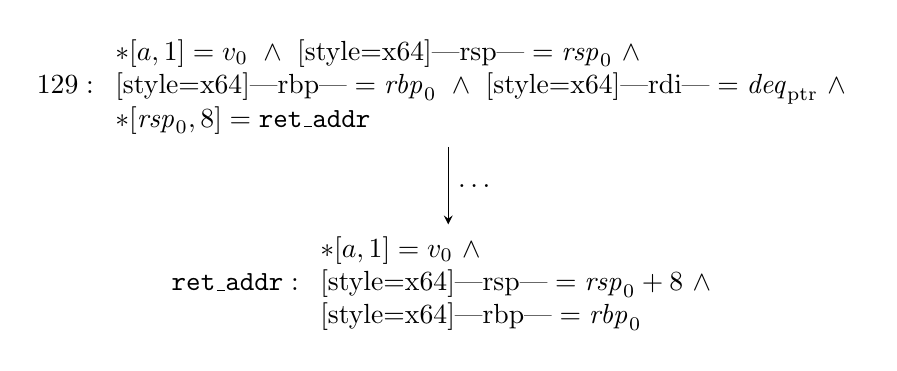
\begin{tikzpicture}[>={stealth}]
      \graph[math nodes, grow down=2.5cm]{
        a/"129:\begin{array}{l}
          \readmem{a}{1} = v_0~\wedge~\mathrsp = \rspo~\wedge \\
          \mathrbp = \rbpo~\wedge~\mathrdi = \deqptr~\wedge \\
          \readmem{\rspo}{8} = \retaddr
        \end{array}" ->[
          "\dots"
        ] b/"\retaddr:\begin{array}{l}
          \readmem{a}{1} = v_0~\wedge\\
          \mathrsp = \rspo + 8~\wedge\\
          \mathrbp = \rbpo
        \end{array}"
      };
    \end{tikzpicture}
    \caption{\lstinline|dequeue_push|}\label{fig:dequeue_push}
  \end{subfigure}
  \begin{subfigure}{.50\linewidth}
    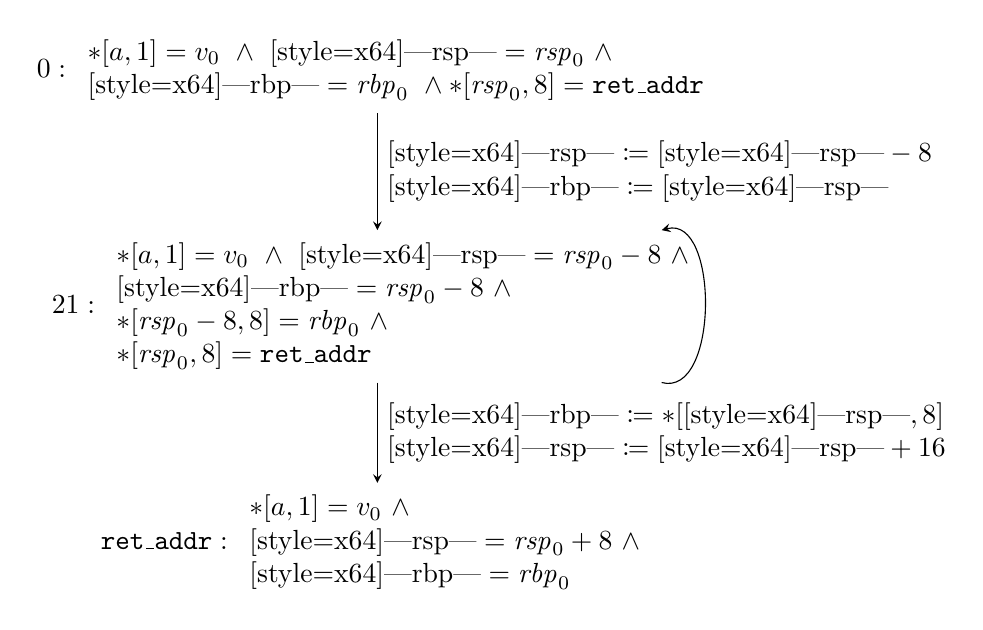
\begin{tikzpicture}[>={stealth}]
      \graph[math nodes, grow down=3cm]{
        a/"0:\begin{array}{l}
          \readmem{a}{1} = v_0~\wedge~\mathrsp = \rspo~\wedge \\
          \mathrbp = \rbpo~\wedge
          \readmem{\rspo}{8} = \retaddr
        \end{array}" ->[
          align=left,
          "$\mathrsp\coloneqq\mathrsp-8$\\
          $\mathrbp\coloneqq\mathrsp$"
        ] b/"21:\begin{array}{l}
          \readmem{a}{1} = v_0~\wedge~\mathrsp = \rspo-8~\wedge \\
          \mathrbp = \rspo-8~\wedge \\
          \readmem{\rspo-8}{8} = \rbpo~\wedge \\
          \readmem{\rspo}{8} = \retaddr
        \end{array}" ->[
          align=left,
          "$\mathrbp\coloneqq\readmem{\mathrsp}{8}$\\
          $\mathrsp\coloneqq\mathrsp+16$"
        ] c/"\retaddr:\begin{array}{l}
          \readmem{a}{1} = v_0~\wedge \\
          \mathrsp = \rspo + 8~\wedge \\
          \mathrbp = \rbpo
        \end{array}";
        b ->[out=-15, in=15, looseness=1] b;
      };
    \end{tikzpicture}
    \caption{\lstinline|buddy_large_avail|}\label{fig:buddy_large_avail}
  \end{subfigure}
  \caption{Example Floyd invariants}
\end{figure*}

\section{Limitations}
% TODO

  
  \chapter{Syntax-Driven Verification} % compare to CFG-driven

	\chapter{Conclusions}\label{ch:conclusions}
	\chapter{Summary}\label{ch:summary} % keep?

	\bibliographystyle{plainnat}
	\bibliography{bibliography}

  \clearpage\phantomsection % Getting hyperref to link to the right page
  \printindex

	% This formats the chapter name to appendix to properly define the headers:
	\appendix

	% Add your appendices here. You must leave the appendices enclosed in the appendices environment in order for the table of contents to be correct.
	\begin{appendices}
		\chapter{First Appendix} \label{app:appendix_one}
			\section{Section one} \label{ase:app_one_sect_1}
			\section{Section two} \label{ase:app_one_sect_2}
		\chapter{Second Appendix} \label{app:appendix_two}
	\end{appendices}

\end{document}


%****************************************************************************
% Below are some general suggestions for writing your dissertation:
%
% 1. Label everything with a meaningful prefix so that you
%    can refer back to sections, tables, figures, equations, etc.
%    Usage \label{<prefix>:<label_name>} where some suggested
%    prefixes are:
%			ch: Chapter
%     		se: Section
%     		ss: Subsection
%     		sss: Sub-subsection
%			app: Appendix
%     		ase: Appendix section
%     		tab: Tables
%     		fig: Figures
%     		sfig: Sub-figures
%     		eq: Equations
%
% 2. The VTthesis class provides for natbib citations. You should upload
%	 one or more *.bib bibtex files. Suppose you have two bib files: some_refs.bib and
%    other_refs.bib.  Then your bibliography line to include them
%    will be:
%      \bibliography{some_refs, other_refs}
%    where multiple files are separated by commas. In the body of
%    your work, you can cite your references using natbib citations.
%    Examples:
%      Citation                     Output
%      -------------------------------------------------------
%      \cite{doe_title_2016}        [18]
%      \citet{doe_title_2016}       Doe et al. [18]
%      \citet*{doe_title_2016}      Doe, Jones, and Smith [18]
%
%    For a complete list of options, see
%      https://www.ctan.org/pkg/natbib?lang=en
%
% 3. Here is a sample table. Notice that the caption is centered at the top. Also
%    notice that we use booktabs formatting. You should not use vertical lines
%    in your tables.
%
%				\begin{table}[htb]
%					\centering
%					\caption{Approximate computation times in hh:mm:ss for full order 						versus reduced order models.}
%					\begin{tabular}{ccc}
%						\toprule
%						& \multicolumn{2}{c}{Computation Time}\\
%						\cmidrule(r){2-3}
%						$\overline{U}_{in}$ m/s & Full Model & ROM \\
%						\midrule
%						0.90 & 2:00:00 & 2:08:00\\
%						0.88 & 2:00:00 & 0:00:03\\
%						0.92 & 2:00:00 & 0:00:03\\
%						\midrule
%						Total & 6:00:00 & 2:08:06\\
%						\bottomrule
%					\end{tabular}
%					\label{tab:time_rom}
%				\end{table}
%
% 4. Below are some sample figures. Notice the caption is centered below the
%    figure.
%    a. Single centered figure:
%					\begin{figure}[htb]
%						\centering
%						\includegraphics[scale=0.5]{my_figure.eps}
%						\caption{Average outlet velocity magnitude given an average
%				        input velocity magnitude of 0.88 m/s.}
%						\label{fig:output_rom}
%					\end{figure}
%    b. Two by two grid of figures with subcaptions
%					\begin{figure}[htb]
%						\centering
%						\begin{subfigure}[h]{0.45\textwidth}
%							\centering
%							\includegraphics[scale=0.4]{figure_1_1.eps}
%							\caption{Subcaption number one}
%							\label{sfig:first_subfig}
%						\end{subfigure}
%						\begin{subfigure}[h]{0.45\textwidth}
%							\centering
%							\includegraphics[scale=0.4]{figure_1_2.png}
%							\caption{Subcaption number two}
%							\label{sfig:second_subfig}
%						\end{subfigure}
%
%						\begin{subfigure}[h]{0.45\textwidth}
%							\centering
%							\includegraphics[scale=0.4]{figure_2_1.pdf}
%							\caption{Subcaption number three}
%							\label{sfig:third_subfig}
%						\end{subfigure}
%						\begin{subfigure}[h]{0.45\textwidth}
%							\centering
%							\includegraphics[scale=0.4]{figure_2_2.eps}
%							\caption{Subcaption number four}
%							\label{sfig:fourth_subfig}
%						\end{subfigure}
%						\caption{Here is my main caption describing the relationship between the 4 subimages}
%						\label{fig:main_figure}
%					\end{figure}
%
%----------------------------------------------------------------------------
%
% The following is a list of definitions and packages provided by VTthesis:
%
% A. The following packages are provided by the VTthesis class:
%      amsmath, amsthm, amssymb, enumerate, natbib, hyperref, graphicx,
%      tikz (with shapes and arrows libraries), caption, subcaption,
%      listings, verbatim
%
% B. The following theorem environments are defined by VTthesis:
%      theorem, proposition, lemma, corollary, conjecture
%
% C. The following definition environments are defined by VTthesis:
%      definition, example, remark, algorithm
%
%----------------------------------------------------------------------------
%
%  I hope this template file and the VTthesis class will keep you from having
%  to worry about the formatting and allow you to focus on the actual writing.
%  Good luck, and happy writing.
%    Alan Lattimer, VT, 2016
%
%****************************************************************************
